\section{数据处理}
\subsection{数据获取}
通过Python爬虫获取了1月20日至今的疫情数据。
此处确诊与重症均为去除死亡人数的数值。
\\
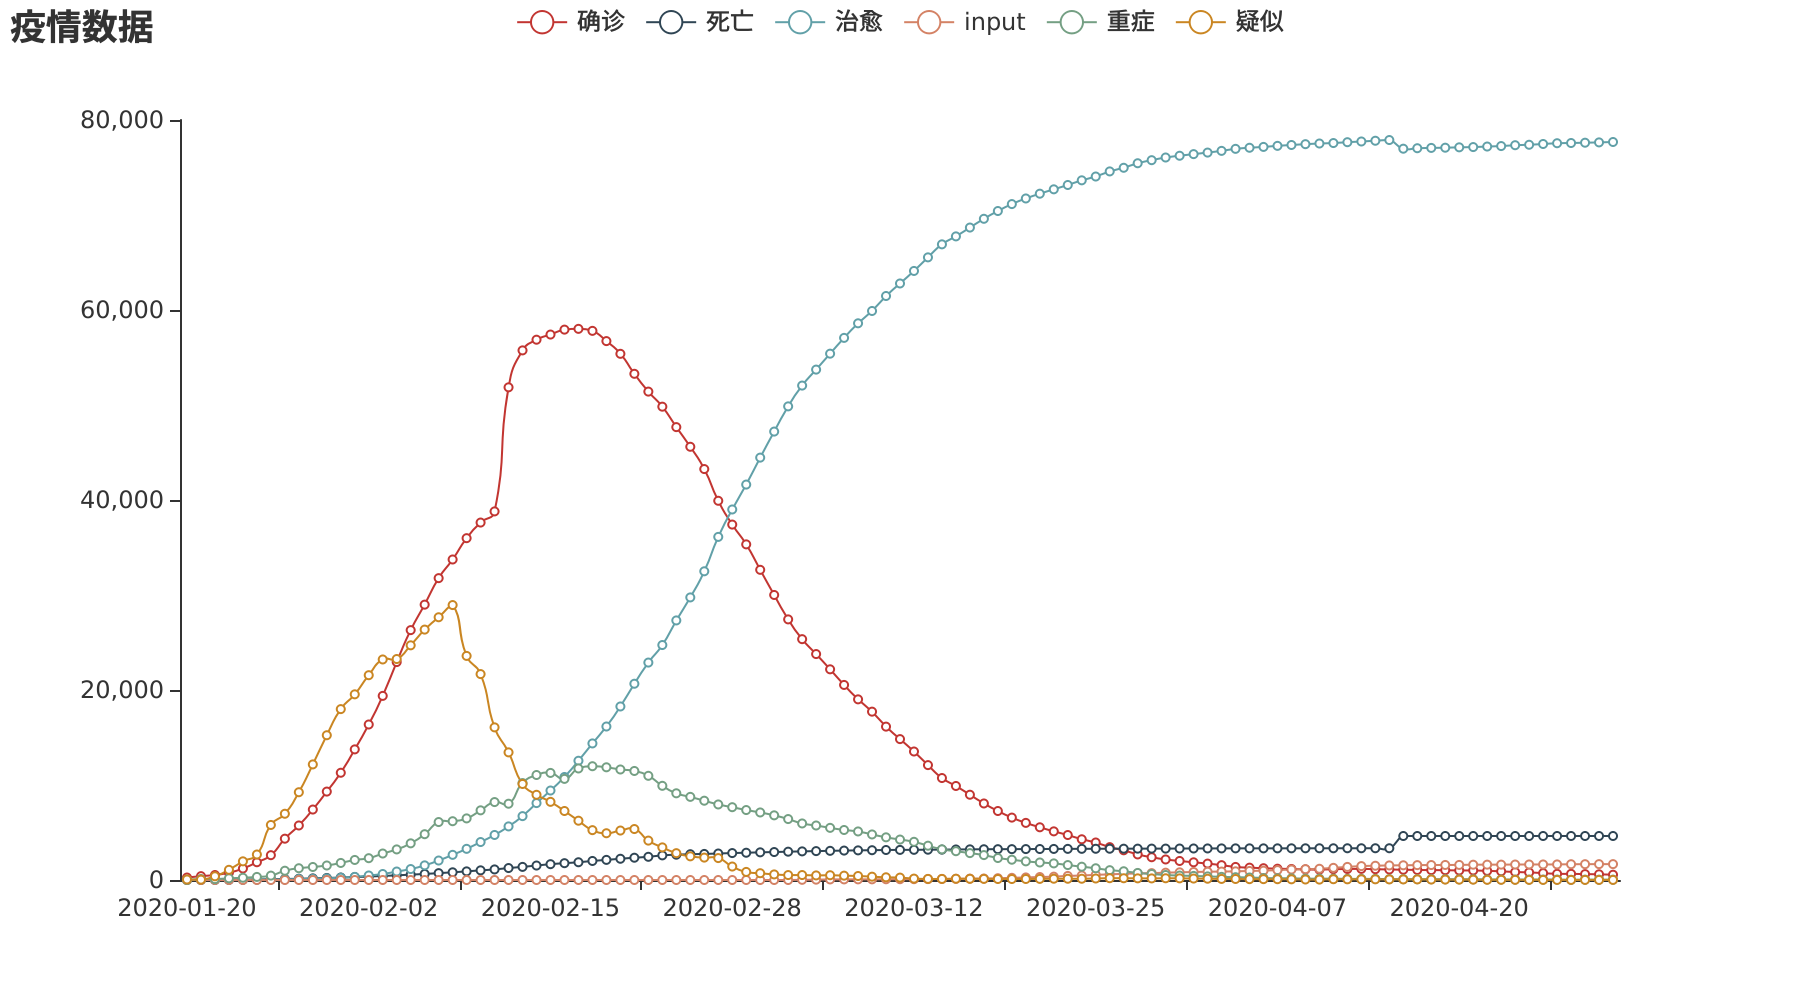
\includegraphics[width=\imagewidth]{疫情数据.png}
\par
可见治愈曲线相较确诊及疑似曲线明显滞后。
\subsection{数据分析}
对数据进行简单的处理,得到每日新增人数曲线。
\\
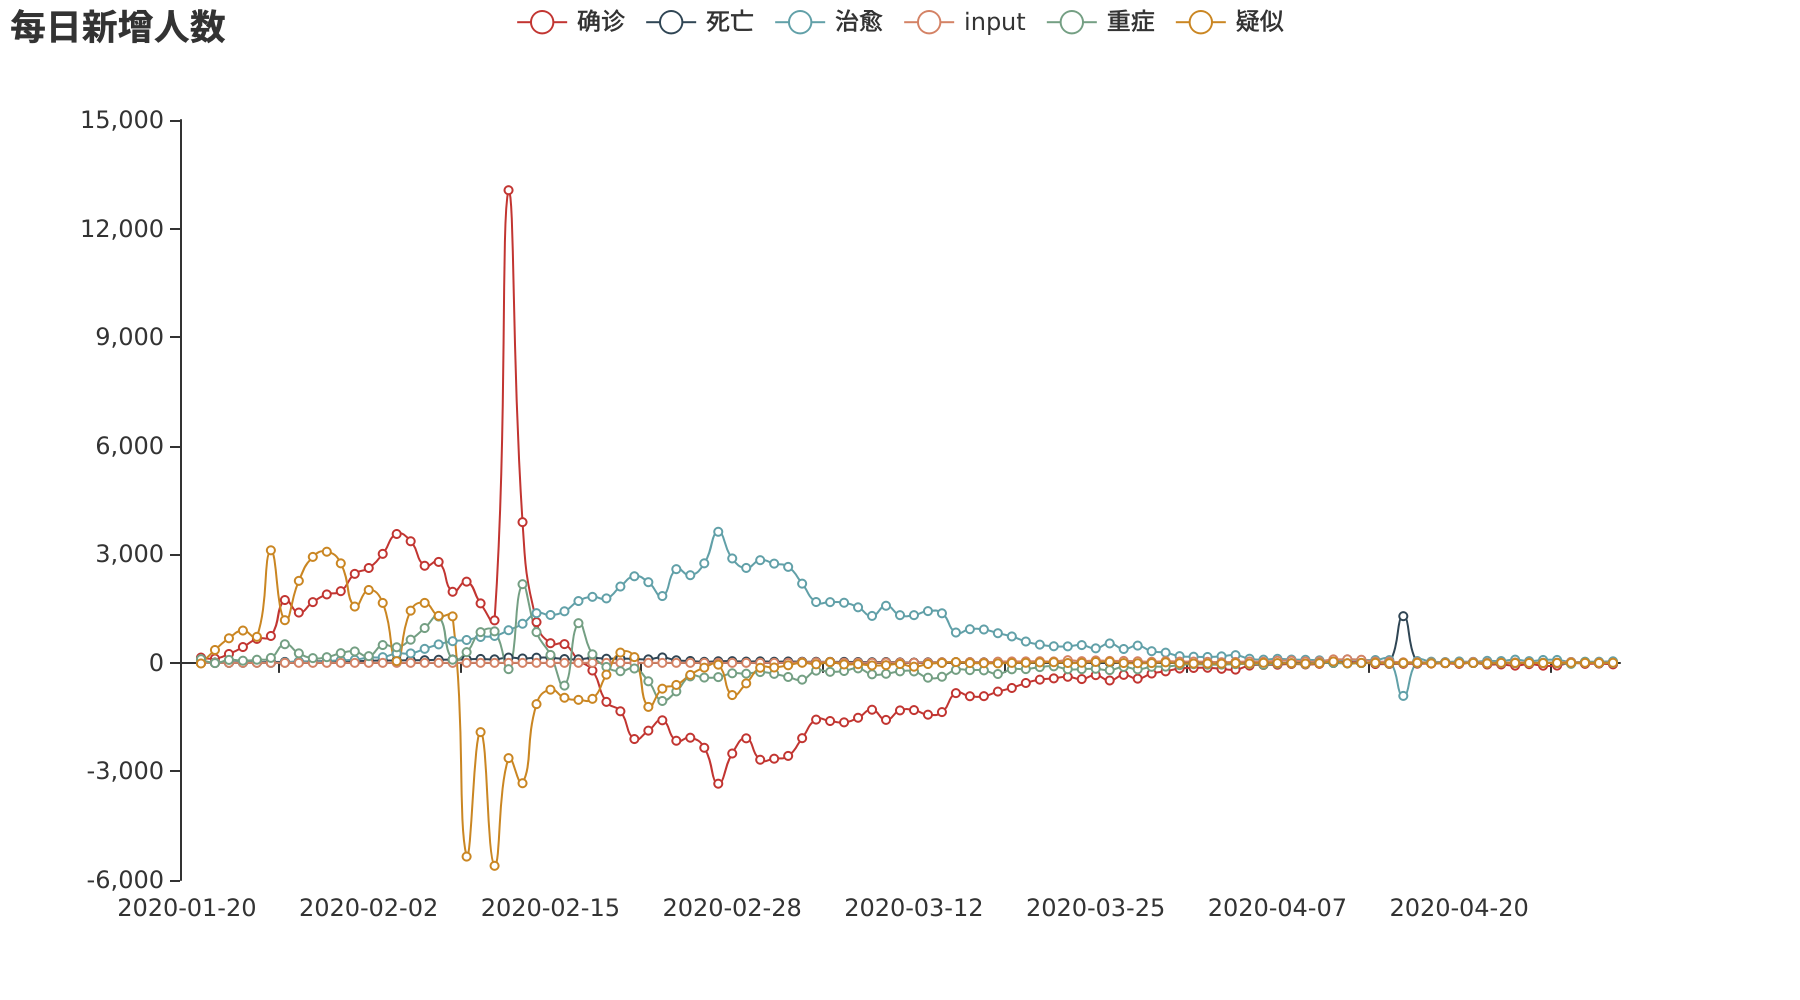
\includegraphics[width=\imagewidth]{每日新增人数.png}
\par
对数据进行简单的观察,可见2月12日确诊人数猛增,
这是因为重新规定了确诊条件,导致许多人被纳入确诊人数。
\par
通过确诊死亡比例可以大致判断致死率。
\\
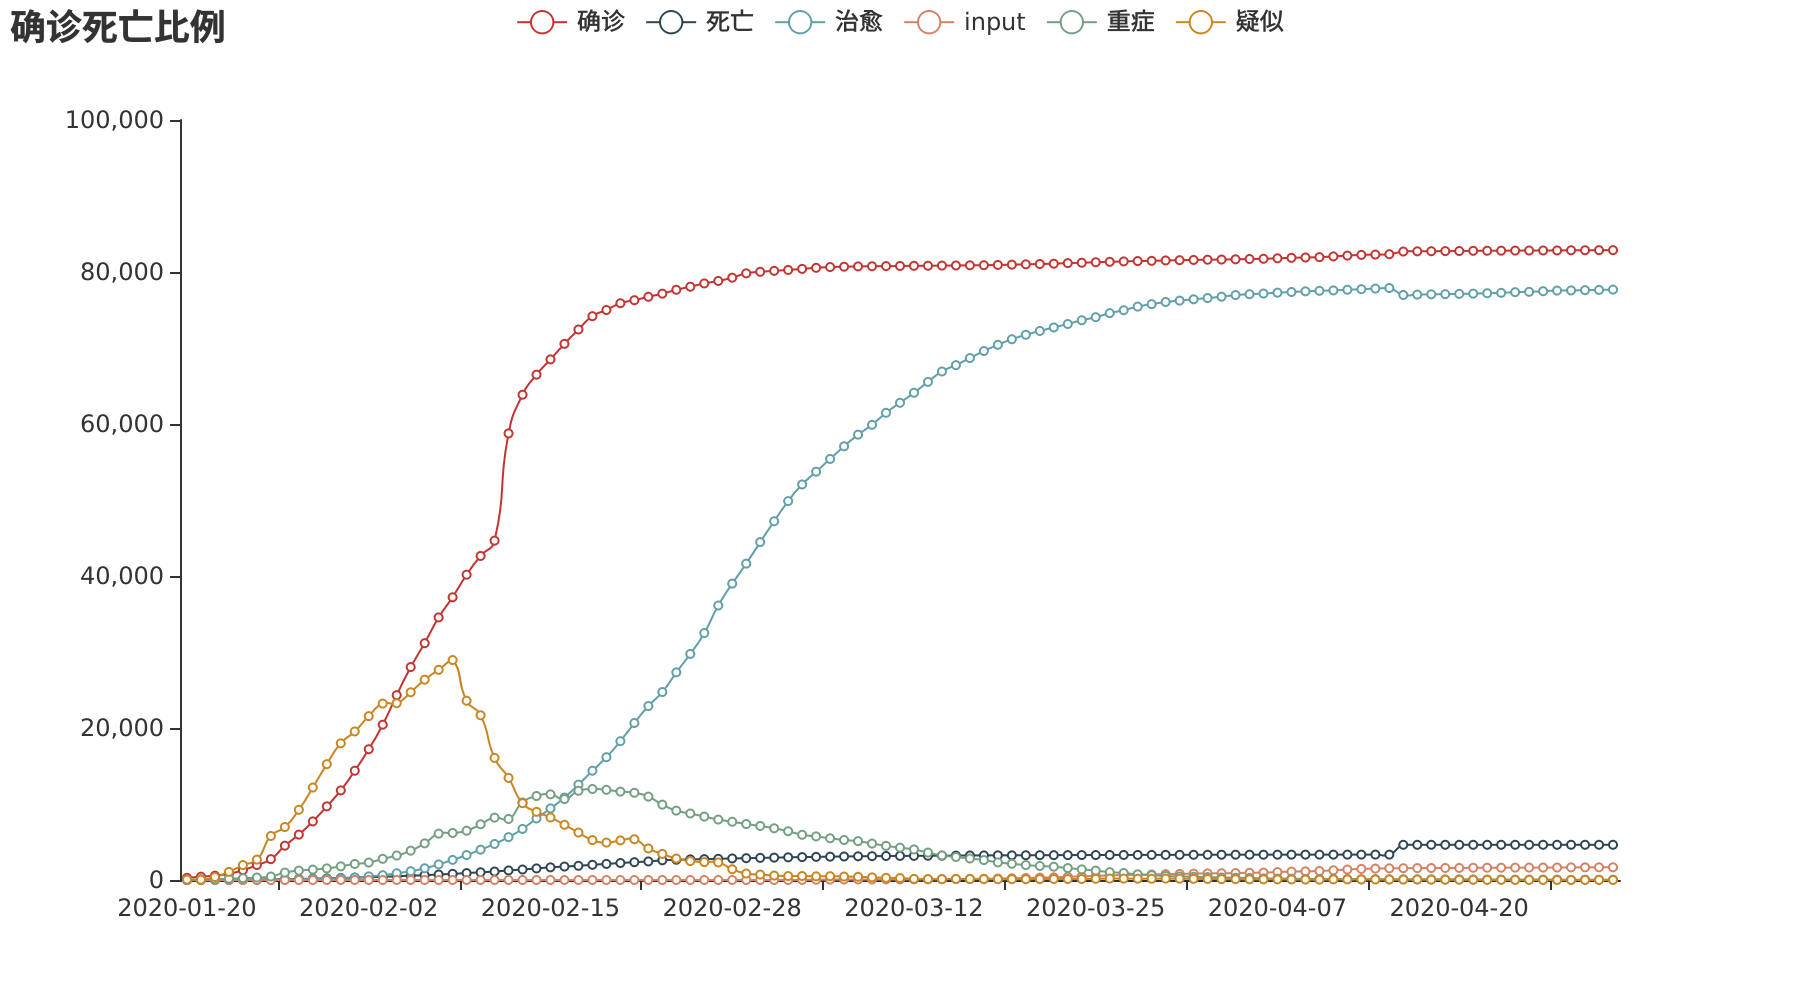
\includegraphics[width=\imagewidth]{确诊死亡比例.png}
\par
可见死亡比例在$0.2\sim 0.5$间波动,最终稳定于$0.5$。
\\
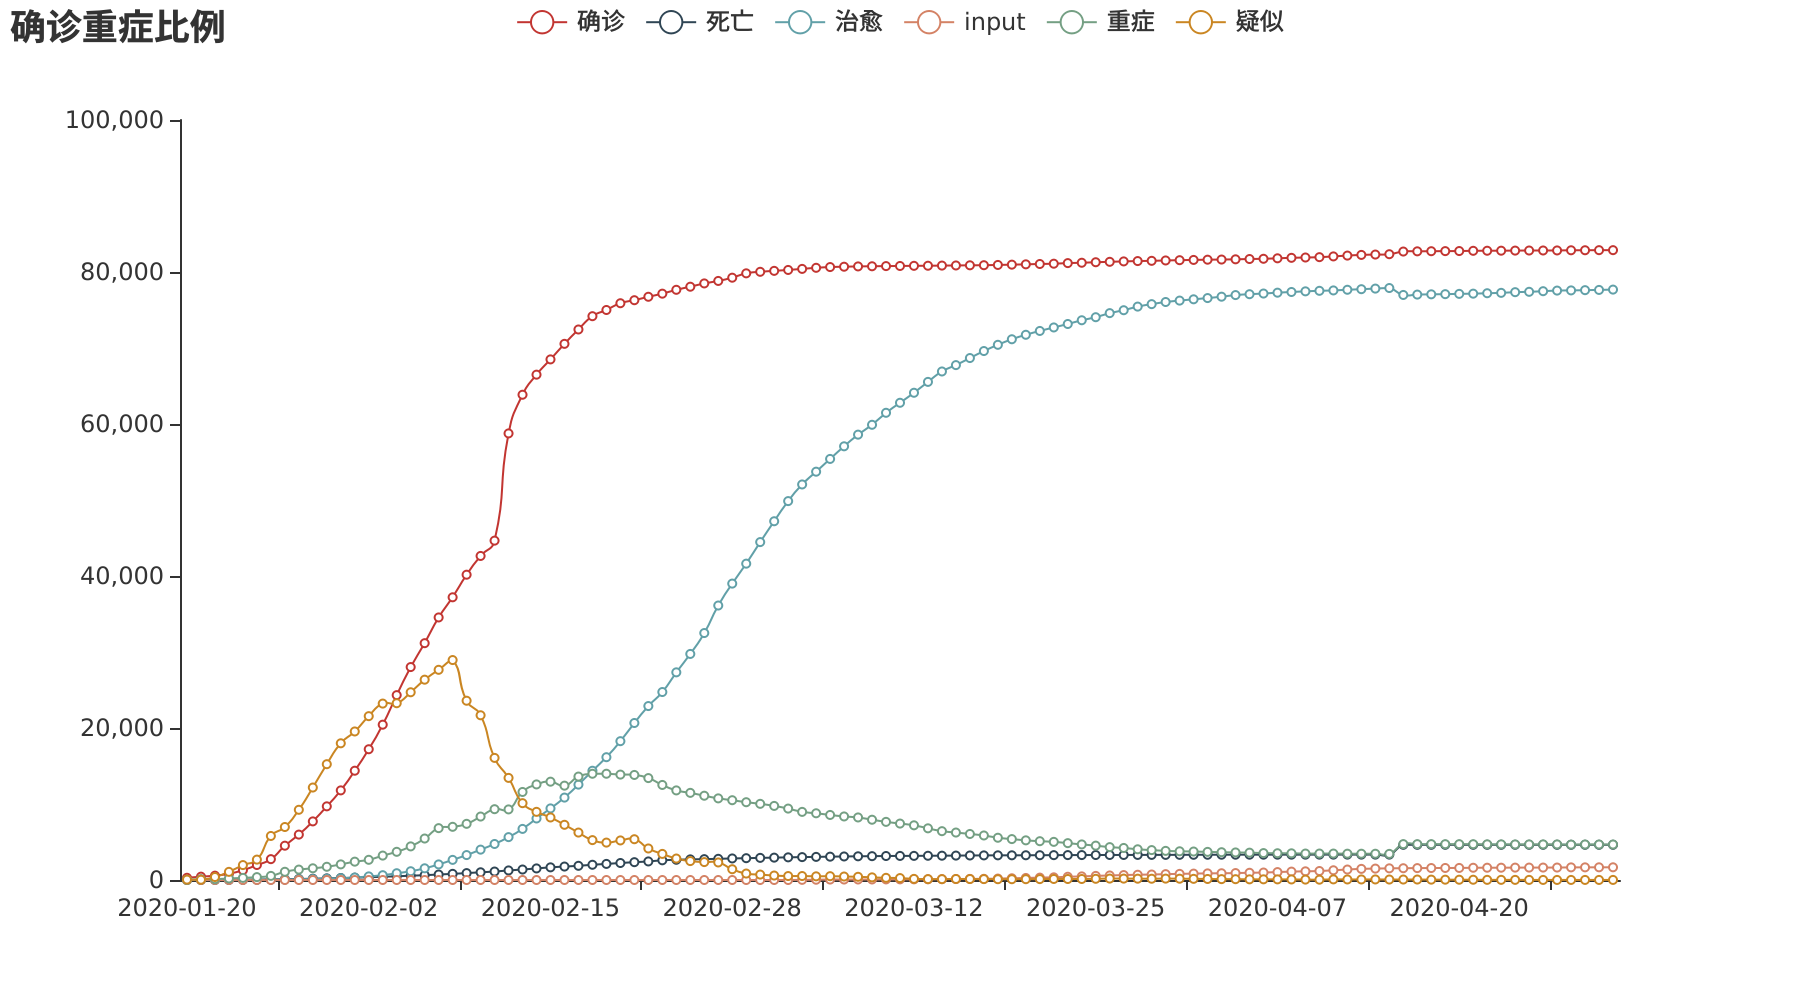
\includegraphics[width=\imagewidth]{确诊重症比例.png}
\par
可知,自2月中旬起,重症比例逐步下降。
\\
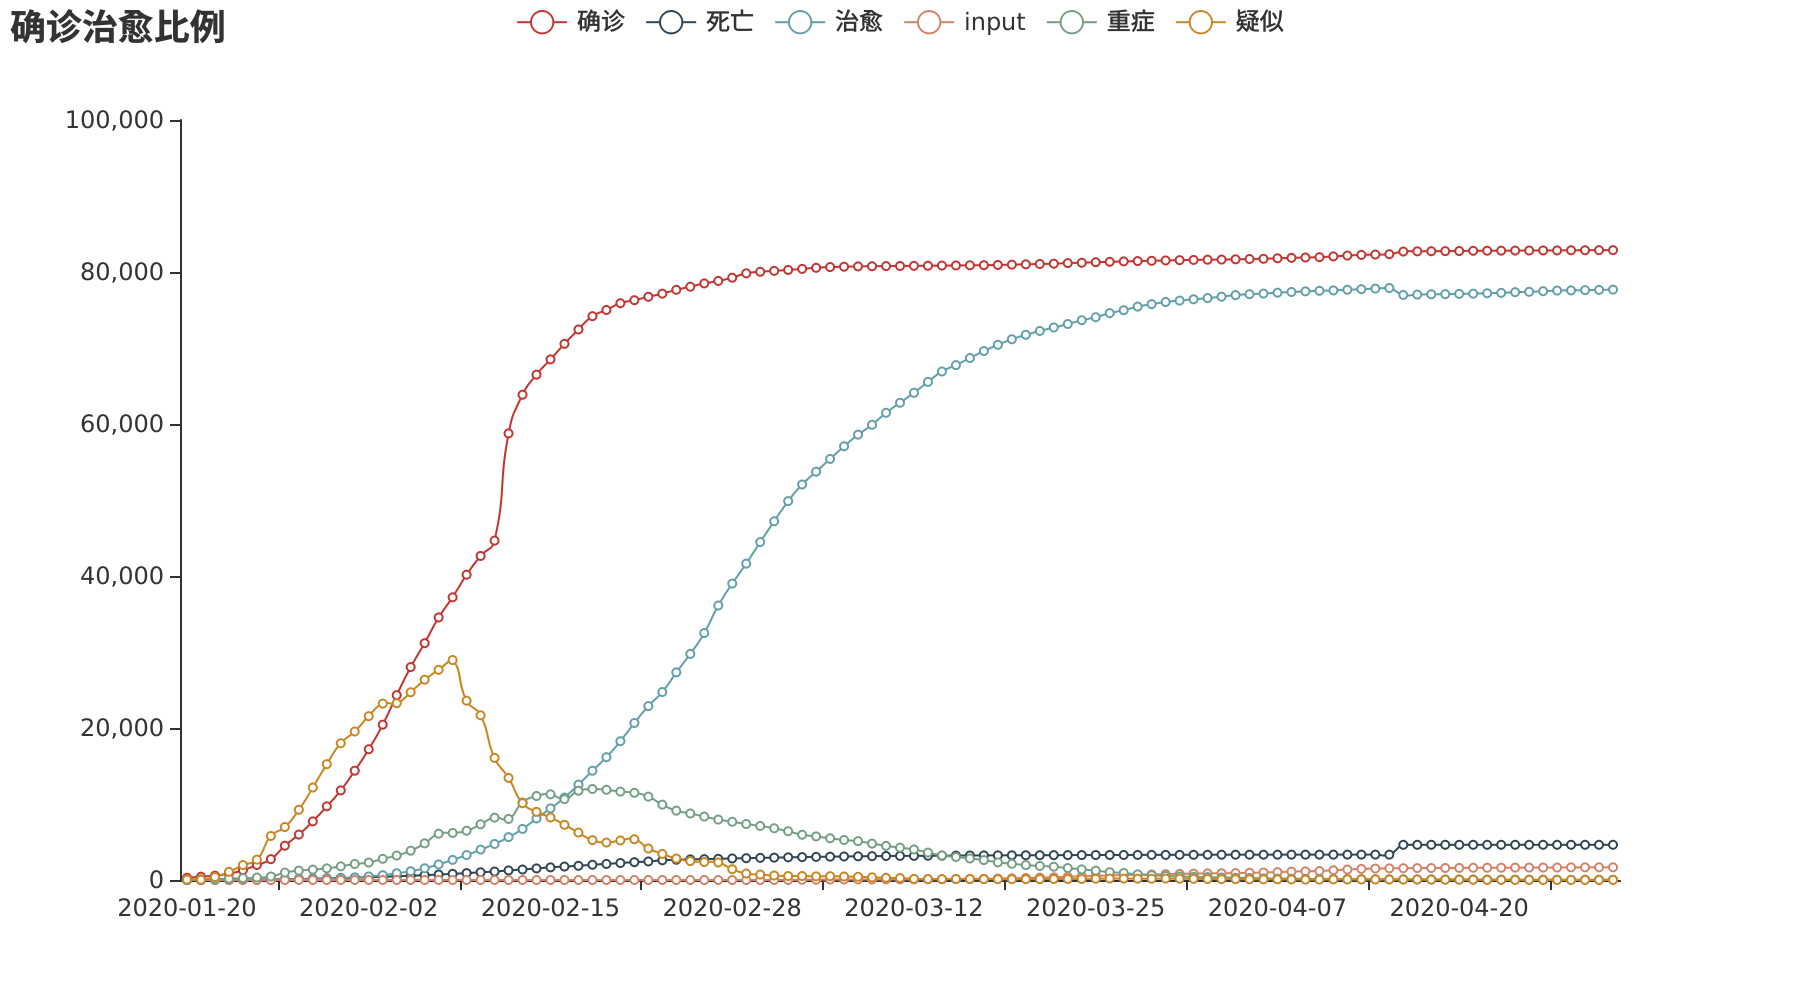
\includegraphics[width=\imagewidth]{确诊治愈比例.png}
\par
可见治愈率越来越高,大体呈$logtic$回归趋势。

